\begin{frame}
    \begin{definition}
        An embedded system is a computer system --- a combination of computer processor, computer memory, and input/output peripheral devices --- that has a dedicated function within a larger mechanical or electronic system (Source: \href{https://en.wikipedia.org/wiki/Embedded_system}{Wikipedia - Embedded Systems}).
    \end{definition}
    \vspace{-1em}
    \begin{figure}
        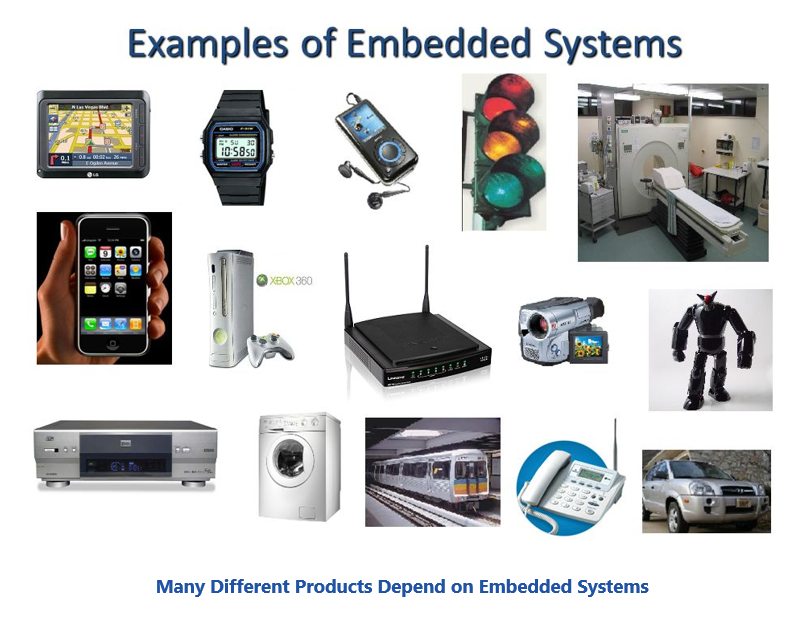
\includegraphics[width=0.5\textwidth]{microcontroller/embedded-system-examples.png}
        \caption{\glsentrydesc{es} examples}
    \end{figure}
\end{frame}